%-----------------------------------------------------------------------------
%
%               Template for sigplanconf LaTeX Class
%
% Name:         sigplanconf-template.tex
%
% Purpose:      A template for sigplanconf.cls, which is a LaTeX 2e class
%               file for SIGPLAN conference proceedings.
%
% Guide:        Refer to "Author's Guide to the ACM SIGPLAN Class,"
%               sigplanconf-guide.pdf
%
% Author:       Paul C. Anagnostopoulos
%               Windfall Software
%               978 371-2316
%               paul@windfall.com
%
% Created:      15 February 2005
%
%-----------------------------------------------------------------------------


\documentclass[10pt, numbers, preprint ]{sigplanconf}

% The following \documentclass options may be useful:

% preprint      Remove this option only once the paper is in final form.
% 10pt          To set in 10-point type instead of 9-point.
% 11pt          To set in 11-point type instead of 9-point.
% numbers       To obtain numeric citation style instead of author/year.
%\usepackage[colorlinks, linkcolor=black, anchorcolor=black, citecolor=black]{hyperref}
\usepackage{hyperref}
\hypersetup{hidelinks}
\usepackage{amsmath}
\usepackage{graphicx}
\usepackage{textcomp}
\usepackage{url}
\def\UrlBreaks{\do\A\do\B\do\C\do\D\do\E\do\F\do\G\do\H\do\I\do\J
\do\K\do\L\do\M\do\N\do\O\do\P\do\Q\do\R\do\S\do\T\do\U\do\V
\do\W\do\X\do\Y\do\Z\do\[\do\\\do\]\do\^\do\_\do\`\do\a\do\b
\do\c\do\d\do\e\do\f\do\g\do\h\do\i\do\j\do\k\do\l\do\m\do\n
\do\o\do\p\do\q\do\r\do\s\do\t\do\u\do\v\do\w\do\x\do\y\do\z
\do\.\do\@\do\\\do\/\do\!\do\_\do\|\do\;\do\>\do\(\do\)\do\,
\do\?\do\'\do+\do\=\do\#}

\newcommand{\cL}{{\cal L}}

\begin{document}

\special{papersize=8.5in,11in}
\setlength{\pdfpageheight}{\paperheight}
\setlength{\pdfpagewidth}{\paperwidth}

%\conferenceinfo{VEE '18,}{April 08-09, 2018, Xi'an, China}
%\copyrightyear{2017}
%\copyrightdata{978-1-4503-4948-2/17/04}
%\copyrightdoi{3050748.3050767}

% Uncomment the publication rights you want to use.
%\publicationrights{transferred}
%\publicationrights{licensed}     % this is the default
%\publicationrights{author-pays}

\titlebanner{}        % These are ignored unless
\preprintfooter{}   % 'preprint' option specified.

\title{HyperPS: A VM Protection System against Compromised Hypervisor Based on Privilege Separation}
\authorinfo{Kunli Lin$^1$$^2$\and Kun Zhang$^1$$^2$\and Haojun Xia$^1$$^2$\and Bibo Tu$^1$$^2$ }
           {$^1$Institute of Information Engineering, Chinese Academy of Sciences, Beijing\\
            $^2$School of Cyber Security, University of Chinese Academy of Sciences, Beijing\\
          {\{tubibo\}@iie.ac.cn}

\maketitle

\begin{abstract}
Hypervisor lays the foundation stone of cloud computing. Once the hypervisor is compromised, all user's virtual machines (VMs) running on it are at risk. To solve this problem, some researchers propose the hypervisor with small code size to shrink its large attack surface. Others introduce a more privileged software or hardware layer to monitor the vulnerable hypervisor. Compared with protecting the vulnerable hypervisor, VM protection mechanisms that do not rely on the security of the hypervisor are more attractive.

In this paper, we propose a novel approach, named HyperPS to separate the fundamental and crucial privileges of the hypervisor into a new trusted environment (T-monitor) against compromised hypervisor, which does not require any software/hardware of higher privilege than hypervisor. A pivotal condition for HyperPS is that reconstructed hypervisor is no longer possible to operate security-sensitive system resources. To operate security-sensitive resources, hypervisor must to request the T-monitor to perform it. We have implemented a prototype for KVM hypervisor on x86 platform with multiple VMs running Linux, which can be applied to current commercial cloud computing industry. Experiment data shows that our approach can provide a VM protection system against attacks with negligible performance influence.
\end{abstract}

%\category{D.4.6}{Operating Systems}{Security and Protection}

%general terms are not compulsory anymore, you may leave them out
%\terms
%Design, Security, Performance

\keywords
Cloud Computing, Virtualization, Hypervisor, VM Security, Memory Isolation

\section{INTRODUCTION}
\label{sec:introduction}%在云环境中Hypervisor扮演了举足轻重的角色,进行物理资源管理和抽象,将资源分配给每个虚拟机。为了对内存和处理器进行抽象,Hypervisor定义了VCPU和二级页表映射。
In cloud, the task of the hypervisor or VMM (virtual machine monitor) is to allocate resource for the virtual machines(VMs) in addition to providing interfaces for higher level administration and monitoring tool\cite{perez2013characterizing}. The hypervisor that has full control of the system runs at the highest privilege level. The hypervisor usually uses some important data structures to manage all guest virtual machines (VMs). In virtualized environments, vCPU (virtual CPU) as the logical abstraction of the physical CPU, \cite{hai2011virtual} is described as an important data structure: Virtual-Machine Control Structure (VMCS). The VMCS defines what kind of operations the VM can conduct, the conditions that can trigger VM exits, and the operations that the hypervisor can conduct when vm exits. %(对VMCS的表达不确切。页表:x86架构下是intel EPT和amd NPT)
Extended page table (EPT)\cite{epturl}/Nested Page Table (NPT)\cite{mijat2011virtualization}/Shadow Page Table(SPT)\cite{shadowpturl} in charge of translation between guest physical memory and host physical address.

Although the hypervisor has the highest privilege, it may also be compromised by internal administrators and external attackers. %(for example ...)下面应该按照先将威胁分为内部和外部两类,内部可以通过什么攻击实现,有什么特色。外部能够通过什么方式实现,有什么特色。
Once the hypervisor is compromised, the VMs running on it are in danger. As shown in figure\ref{fg1_attk_aprch}, the internal administrators can inject malicious code through management tools to conduct attacks. In the virtualized platform, the VMs are managed by management tools, and the behavior of internal administrators is not limited by firewalls and intrusion detection systems. And internal administrators can send DMA requests through malicious code to perform attacks. They can tamper with or steal code and data in physical memory through DMA devices to implement code injection, control flow hijacking, data leakage and so on. Meanwhile, the internal administrators that have many privileges also can directly modify the kernel page table that provides the mapping between the guest address and physical address. %管理员如何直接修改页表呀?guest address是什么呀,physical address又是指的什么,要明确。还有DMA攻击举一个恰当的例子。内部和外部攻击的效果可能差不多,但是内部更容易实施攻击,并且攻击方式更多样。
Through the kernel page table, they can get crucial information of VMs leading to information leakage. And external attackers can exploit the software vulnerability of hypervisor to attack the VMs, even the attackers can hire a VM on the same physical server to attack other VMs. As shown in the figure \ref{fg1_attk_aprch}, external attacks have at least two ways to threaten the security of the VM. One is to get the permissions of the hypervisor through the VM escape attack, so that the malicious code can be injected to destroy the security of the critical data structure to threaten the security of the VM. Another way is to compromise the security of the VM through the VM's dual mapping attack and remapping attack.
%虚拟机逃逸是一种攻击,而remapping attack也是通过逃逸后才能实施。外部攻击的分析不到位。
%所有图片的分辨率太低,线条和字体都已失真
\begin{figure}[htbp]
	\centerline{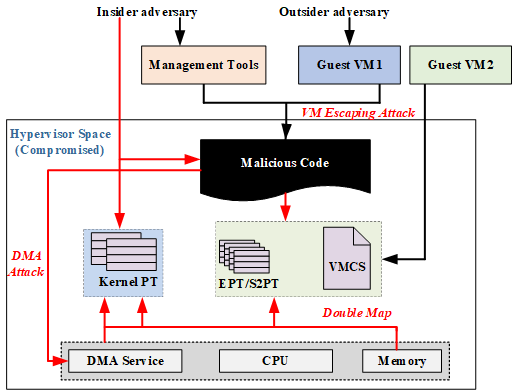
\includegraphics[height=2.00in]{figures/p1.png}}
	\caption{Attack path.}
	\label{fg1_attk_aprch}
\end{figure}

In light of these attacks, there is a pressing need to investigate effective ways to guarantee VM security once the hypervisor is compromised. Privilege separation\cite{DBLP:conf/ndss/ChoKYP17, murray2008privilege, burdonov2009virtualization, chen2011linux} has been considered as a fundamental principle that can separate the critical capability from the hypervisor and remove such a security concern. In order to reduce the threat to other components or the whole system caused by attackers, and enforce this security principle in the design, current researchers try to alleviate those vulnerabilities by hardware or software on a higher level than the hypervisor.

%引用可以直接用cite{sgx1, sgx2, sgx3}
\textbf{Hardware features.} Different hardware platforms provide different hardware mechanisms, such as Intel’s Software Guard Extensions (SGX)\cite{sgx1} \cite{sgx2} \cite{sgx3} and AMD’s Secure Memory Encryption (SME)\cite{DBLP:conf/hpca/WuLLCZG18}. SGX provides protection for pieces of application logic inside encrypted enclave memory against malicious OS. However, it is limited to protect a relatively small portion of memory, and the developers have to mostly reconstruct the protected software or build it from scratch\cite{sgxexplain}. Therefore it is nontrivial for SGX to protect large-scale software like the entire VM. SME can encrypt memory in page level granularity by simply setting the C-bit in the page table entry. %SME是一台物理机利用一个密钥,不能防护跨域攻击,只能防护cold boot attack. SEV是每个VM一个密钥,密钥Hypervisor并不能得知,即使remapping也无济于事
More importantly, AMD enables the Secure Encrypted Virtualization (SEV) feature\cite{}. However, a malicious hypervisor can bypass the protection by manipulating some critical resources, such as guest memory mapping and key sharing mechanisms.
%上面是商业CPU带的特性,可以加入一些基于硬件安全的学术论文,如Bastion、secureme等

\textbf{Software at Higher Privilege Level.} In order to mitigate the hazard caused by the hypervisor, plenty of software solutions are proposed which introduce a higher privilege-level layer than the hypervisor. Nested virtualization is one of the representative approaches, which provides a higher-privileged and isolated execution environment to run a monitor securely. The turtles project\cite{DBLP:conf/osdi/Ben-YehudaDDFHGLWY10} and CloudVisor\cite{DBLP:conf/sosp/ZhangCCZ11} are examples that propose nested virtualization idea to achieve isolation for protected resources. To be specific, CloudVisor uses nested virtualization to decouple resource management into the nested hypervisor to protect VMs.

In practice, the independence on platforms and minimum changes to existing systems are the most prized features for cloud providers. For this purpose, some recent efforts introduce software-based approaches that achieve the same privilege-level isolation and protection instead of relying on a higher privilege level.%嵌套虚拟化对原有系统的更改更小,只是加入了一个软件层,原有软件几乎无修改,而基于同层隔离的是要对原有软件进行修改的。应该从性能角度分析,说嵌套虚拟化会有多层上下文切换,操作路径多,性能差。
%同层隔离可以举例说明,并指出其主要针对于arm平台。

In this paper, we introduce a novel prototype, named HyperPS, to protect the security of guest virtual machines running on a compromised hypervisor based on privilege separation without relying on a higher privileged software or microhypervisor.

HyperPS creates a new set of page tables based on the original page tables and implements a security world at the same layer as Hypervisor. The cricual data structures of the hypervisor are put in this security world. Based on this idea, HyperPS implements the hypervisor monitoring and VM memory isolation.

%VMCS和EPT只是其中比较重要的,IOMMU和registers也是要保护的,各种控制寄存器等
Hypervisor monitoring safeguards key data structures including EPT and VMCS, so as to avoid malicious attacks causing the whole system compromised.

%这个文章有两个技术点,一个是做了一个监控框架,将Hypervisor分开成两个,然后是一个保护机制,如果通过限制对敏感资源的访问来保护VM。1 实现同层分离的技术点;2实现VM保护的技术点
The VM memory isolation can resist malicious VM memory accessing from compromised hypervisor and others VMs, especially, remapping and double mapping attack. Firstly, HyperPS marks each page with page marking technique to guarantee each page can only be owned by a single VM. Secondly, it deprives address translation function of the hypervisor to ensure that the page is marked with the owner when it is mapped. Finally, since any update to guest page table can be synced to EPT, HyperPS verifies whether any protected virtual addresses is double mapped or remapped. In order to avoid double mapping attack, the owner of the page is verified when EPT updates. In order to resist remapping attack, HyperPS clears the content of the page when it is released.

It has applicability for multi-platforms (x86, mips and so on), few modifications for the original hypervisor, and practicability for cloud providers. We take x86 architecture as an example. Our prototype introduces 4K SLOC (Source Lines of Code) to VM protection and 300 SLOC modifications of the hypervisor. The experimental results show trivial performance overhead and independence on multi-platforms for runtime VM protection.
%实验环境不能够体现多平台支持

%安全框架单列出来,安全框架不仅可以保护内存,也可以做host完整性和访问控制等。它只是一个TEE,相当于软件实现的TrustZone
Our contributions are as follows:
\begin{itemize}
\item A secure isolated execution environment placed at the same privilege level with hypervisor instead of relying on a higher privilege-level or hardware.
\item A non-bypassable protection approach for VMCS and EPT which can ensure the security of interaction between VM and hypervisor as well as VM memory mapping.
\item An approach of isolating memory among VMs and hypervisor securely for VM by using page marking technique to avoid malicious access from compromised hypervisor.
\item A prototype based on x86 KVM with trivial performance overhead, high security and hardware independence.
\end{itemize}

The rest of this paper is organized as follows. Section \ref{sec:bkground} provides the necessary background background. Section \ref{sec:threatmdasmp} discusses our threat model and assumption. Section \ref{sec:dsgnimplmt} elaborates on the design and implementation of HyperPS on x86 platform. Section \ref{sec:evalu} presents our experimental evaluation of security and performance. Section \ref{sec:relatwk} compares HyperPS with previous work. At last, Section \ref{sec:conclsn} gives the conclusion.

\section{BACKGROUND} \label{sec:bkground}
In this section, we mainly describe related technologies of hypervisor.

%1.内存管理(EPT和hypervisor地址空间);2.vCPU与CPU关联关系,VM Exit和entry;3.TEE介绍下也可以。介绍后续要用到的修改、配置等,有图做辅助
\subsection{VMCS} \label{subsec:vmcs}
Virtualization technique imports two kinds of operation mode, Root and Non-root mode. To better support CPU virtualization, VMCS structure, a data structure based on hardware, is imported to manage transitions out and into of VMX Nonroot mode from VMX Root mode (VM Exit and VM Entry), as well as processor behavior. This structure is divided into six information fields, including Guest-state filed which records VM information and Host-state filed which records host OS information. It causes VM Exit that the vCPU switches from root mode to non-root mode. The reverse operation is called VM Entry that transiting from non-root mode to root mode. During these two operations, VMCS is used primarily for vCPU to query and update key CPU information such as system privileged registers.

\subsection{VM Exit/VM Entry} \label{subsec:vmexit}
VM Exit is primarily due to that the VM has some sensitive instructions that cannot be performed properly and requires hypervisor’s assistance to complete sensitive instruction execution. After VM Exit is finished, CPU needs to execute VMLAUNCH/VMRESUME instruction to initiate VM Entry. The interaction that is triggered by VM Exit process from the VM to hypervisor is as follows. The execution flow of VM Entry is opposite to that of VM Exit.
\begin{enumerate}
\item VM makes interrupt request for VM Exit, and the CPU in non-root mode first records VM Exit reason to the corresponding information filed in VMCS and saves the CPU state to the Guest-state filed of VMCS.
\item The CPU accesses the Host-state filed of VMCS and loads it into CPU.
\item The CPU switches from non-root mode to root mode, reads VM Exit reason in VMCS, and jumps to VM Exit handler function entry.
\item CPU initiates VM Entry and run the VM.
\end{enumerate}

\subsection{Address Translation of VM} \label{subsec:addrtrans}%finish这个词。。。;GPA、HPA没有说明;地址转换是MMU自动完成,只有page fault时hypervisor才会维护EPT
The address translation of VM requests two page tables, guest page table and EPT. Guest page table can finish the translation from guest virtual address (GVA) to GPA. Intel’s VT-x provides EPT, which directly supports address translation from GPA to HPA on hardware, which greatly reduces the difficulty of memory virtualization and further improves the performance of memory virtualization.


\section{THREAT MODEL AND ASSUMPTION} \label{sec:threatmdasmp}
In this section, we discuss our threat model and assumption.

\subsection{Threat Model} \label{subsec:thread_md}%first, second是一个维度,third是另一个维度。IO以及DMA要不要防护要界定清楚
We assume that the hypervisor and kernel have been compromised and controlled by the powerful adversary. The adversary can turn off kernel security mechanisms, such as DEP, SMEP, inject code, even tampers page table mappings of memory region, and then implements attacks based on three attack paths, compromising critical interaction data and VM address mapping. First, the adversary can subvert the critical interaction data during the transitions between VMs and the hypervisor. Second, the adversary can tamper values of EPT entry which results in memory corruption attacks, such as remapping attack, double mapping attack and disrupting isolation among EPTs. Third, In virtualization scenario, internal attackers send DMA requests through malicious code to finish malicious attacks. They can tamper with or steal code and data in physical memory through DMA devices to implement code injection, control flow hijacking, data leakage and so on.

\begin{itemize}
\item Modifying the Interaction Data: For the modification of the critical interaction data during the context switching process, attackers can obtain the address of VMCS and modify it, such as HOST RIP, GUEST CR0, EPTP, et al. For example, modifying the value of privilege register, CR0, can close DEP mechanism, and modifying CR4 can close SMEP mechanism.
\item Modifying the Address Mapping of EPT: Modification of EPT entry can result in memory information leakage. There are three attack scenes, double mapping, remapping attack and disrupting isolation among EPTs of VMs.
\end{itemize}

\textbf{Scene 1.} For double mapping attack, attackers control and compromise a VM, then obtain the privilege of hypervisor through VM escape attack, and maliciously access the VMCS structure to obtain the value of EPT Pointer(EPTP). The attack process is as shown in Figure \ref{fg2_expr_dbmp_atk}. There are two guest VMs, VM1 (attacker) and VM2 (victim). In this way, EPTP of VM1 and EPTP of VM2 are respectively obtained by attackers. Also, for a guest virtual address (GVA) in VM2, named ’A’, is mapped to the corresponding real physical address, named’B’. For VM1, the real physical address corresponding to the guest virtual address ’C’ is ’D’, then ’D’ is modified to be ’B’ by modifying the value of the last page item of EPT. At last,’A’ and ’C’ are mapped to the real physical address ’B’, no address is mapped to ’D’. Then VM1 can access the data of VM2 successfully through accessing ’B’, this attack process is called double mapping attack.

\begin{figure}[htbp]
	\centerline{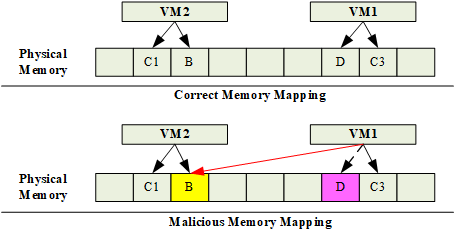
\includegraphics[height=1.80in]{figures/p2.png}}
	\caption{The execution process of double mapping attack.}
	\label{fg2_expr_dbmp_atk}
\end{figure}

\textbf{Scene 2.} In a remapping attack scenario, we assume there are two VMs, VM1, a VM controlled by attackers to attack other VMs, VM2, a victimized VM. %句子
 Hypervisor reclaims a physical page (named ‘A’) from VM2 without clearing the data in it. In the subsequent time, VM1 rquests physical page A from the compromised hypervisor. After that, VM1 remaps a GVA (named ’E’) to ’A’. By this way, VM1 can access the content on ’A’ used by VM2 through ’E’, causing information leakage. Through the analysis of these two kinds of attack models, it is necessary to combat with malicious hypervisor.

\textbf{Scene 3.} For the lack of isolation between EPTs of different VMs, the attacker (VM1) who has compromised the hypervisor can access the victim’s memory by snooping VM2’s EPTP.
\begin{itemize}
\item DMA attack. To improve I/O efficiency, DMA allows peripherals to read or write physical memory without the interference of MMU. The DMA attack is mainly divided into three steps: First, the peripherals are modified to embed malicious code; second, the peripherals are deployed to the target host; finally, the malicious code is used to send DMA requests to implement malicious attacks. The internal attacker directly modifies the key information of the kernel and the virtual machine through the DMA device without mapping the EPT table, thereby implementing code injection, control flow hijacking and data leakage and so on.
\end{itemize}

\subsection{Assumption} \label{subsec:assumption}
We make some assumptions. First, we assume hardware resources are trusted including processor, buses, BIOS, UEFI and so on. The trusted boot based on hardware can ensure the security and integrity of bootloaders and hypervisor. The Trusted Computing Base (TCB) contains HyperPS and hardware resources. Second, this paper does not consider denial of service attack (DOS), side channel attack and hardware-based attack, such as cold-boot attack and RowHammer. Third, we assume that there exists no software that runs at a higher privilege level than the hypervisor.

\section{DESIGN AND IMPLEMENTATION} \label{sec:dsgnimplmt}
In this section, we present the design and implementation details of HyperPS.

\subsection{Overview} \label{subsec:overview}
As described in \ref{sec:bkground} and \ref{sec:threatmdasmp} above, hypervisors are vulnerable to internal attackers and external attackers. when the hypervisor is compromised we should restrict the capabilities of the hypervisor to make it be less powerful. If the hypervisor is not trusted, the capability of writing to crucial data structures (VMCS/EPT/REGS) should not be possessed by the hypervisor. So, we should remove these crucial data structures from hypervisor. We proposed HyperPS has realized this idea.

%两个关键技术:提供隔离监控框架;提供虚拟机敏感资源保护
%监控框架分3部分:空间分割、特权解除和空间切换
%虚拟机保护分2部分:敏感资源受控管理、寄存器等上下文保护
HyperPS is designed to provide a secure isolated domain to provide hypervisor monitoring against attackers without depending on a higher privilege-level software than the hypervisor or microhypervisor. Figure \ref{fg3_hyperps} depicts the overview of HyperPS which creates other secure address spaces based on a set of new page table. It is composed of three parts, Normal World, HyperPS World and Switch Gate. A pivotal condition for HyperPS is that Normal World (origin hypervisor) must not be allowed to manipulate any security-sensitive system resources, such as EPT, VMCS, page tables and system control registers. To meet this condition, Normal World is deprived of controlling authority over security-sensitive system resources. Therefore, VMCS and EPT are hidden in HyperPS World from Normal World accessing. Instead, Normal World is only allowed to send requests through a specified interface (Switch Gate) to HyperPS World for controlling these resources. To assess the security of interaction between hypervisor and VM, VM memory mapping, management on VMCS and EPT, are hooked and trapped to HyperPS World. Page table and control register management is used to guarantee the security of HyperPS World. VM Exit redirection can balance VM Exit and VMCS management. Upon receiving such a request, HyperPS World determines whether to accept or reject it. More importantly, only virtual address of Normal World is mapped in page table of Normal World while all virtual address of two worlds is mapped in page table of HyperPS World.

\begin{figure}[htbp]
	\centerline{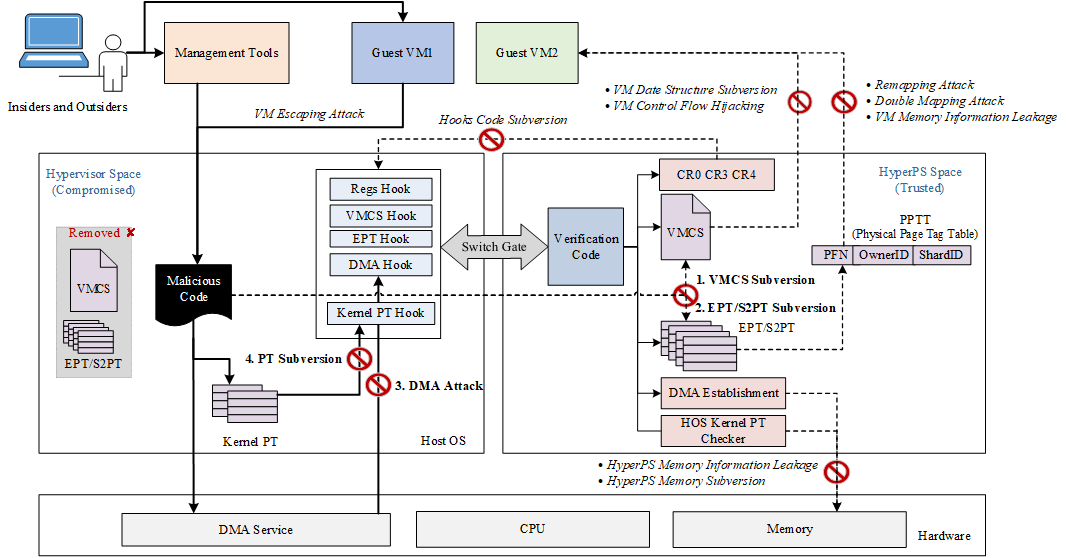
\includegraphics[height=2.50in]{figures/p3.png}}
	\caption{An overview of HyperPS.}
	\label{fg3_hyperps}
\end{figure}

While the hypervisor together with guest VMs runs in Normal World, the hypervisor is forced to request HyperPS to perform two operations on its behalf: 1) switching context between the hypervisor and VMs, 2) updating EPT of VMs, 3) verifying the pages when executing swapping operations to resist double mapping attack, 4) verifying the pages when executing releasing operations to resist remapping attack. With these designs, HyperPS intercepts and monitors VMCS and EPT access, meanwhile, HyperPS enforces the isolation and protection of memory used by each VM. Furthermore, HyperPS guarantees security of interaction and address translation of VMs.

In summary, HyperPS prevents internal attackers from tampering with data structures such as VMCS and EPT, hijacking data streams, and DMA attacks, and prevents remapping and dual mapping of virtual machines.

\subsection{Security-sensitive Resource Access} \label{subsec:secusra}
For the implement, the hypervisor corresponding to Normal World should be modified to be deprived of control capabilities for security-sensitive system resources, including control registers, page table, VMCS and EPT. In order to clarify the resource access in HyperPS World, hooks, unintended instruction elimination and interaction flow are described as follows.

\textbf{Hooks.} We recognize control register access, page table updating, VMCS and EPT operations in Normal World as designated hypervisor events. To tackle the threats from compromised hypervisor, hypervisor monitoring invokes the integrity assessment routines upon the occurrences of designated hypervisor events. A common approach to capture designated events is to place hooks into the origin hypervisor and eliminate related privilege instructions. These hooks can be code hooks (jump instructions) inserted at arbitrary locations in hypervisor code, or any other technique that can transfer the control flow.

\textbf{Unintended Instruction Elimination.} Instructions composed of several fields in x86 are unintended. One or several of these fields may casually match another privileged instruction causing privilege instructions expected to be eliminated retained and hook failure. The general situation is as follows: 1)One instruction contains another privilege instruction. 2)A privilege instruction can be formed across two instructions. There is a threat that attackers jump into the middle of the instructions to execute a privileged instruction which has been eliminated and hooked by us. For the first case, the attack is blocked by replacing the same kind of resource, such as replacing the register in the instruction with another register. The solution to prevent the second attack is that we insert NOP instruction in the middle of these two instructions.

\textbf{Interaction Flow.} When the hypervisor’s execution reaches a hook, it will transfer the control flow to HyperPS World. By implanting hooks at the code positions where hypervisor events occur, HyperPS can capture the occurrences of designated events to assess the sensitive resource integrity.

\subsection{HyperPS World} \label{subsec:hyperpswld}
The creation of HyperPS World has two purposes: 1) creating a address space which can provide monitoring for VMCS and EPT. 2)  creating a software system that does not depend on hardware devices and adapts to multi-system platforms. The key point of its design is that it creates address space used for privilege separation for all privilege levels at the same privilege-level with hypervisor or kernel.

\begin{figure}[htbp]
	\centerline{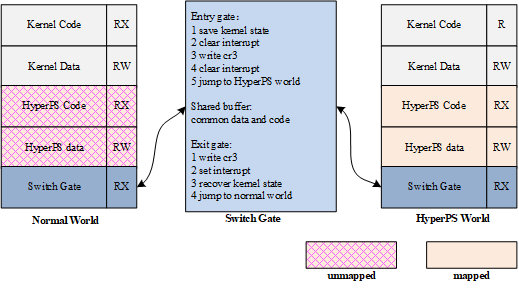
\includegraphics[height=2.00in]{figures/p4.png}}
	\caption{An overview of address space layout.}
	\label{fg4_addr_space}
\end{figure}

\textbf{Creating HyperPS World.} We create another page table to achieve an isolated address space, named HyperPS World, from compromised hypervisor. Figure \ref{fg4_addr_space} describes the address space layout of two worlds through two sets of page tables, the normal page table and HyperPS page table. On the left of Figure \ref{fg4_addr_space}, the normal page table contains code and data of Normal World except for that of HyperPS World. This can prevent compromised hypervisor from breaking the integrity of HyperPS World. Programs running in Normal World cannot access data in HyperPS World. On the right of Figure \ref{fg4_addr_space}, all code and data segments are mapped in HyperPS page table. HyperPS code remains executable and HyperPS data remains writable. What’s the most important, kernel code is forbid to execute when HyperPS World is active, so that it cannot attack HyperPS World.

\textbf{Creating Switch Gate.} HyperPS designs and implements Switch Gate to perform worlds switching by executing a series of ordinary instructions. Switch Gate performs the control switching operation between Normal World and HyperPS World, acting as a wrapper function for a handler which processes incoming requests in HyperPS World. It provides Normal World with a unique way to enter HyperPS World. In addition, Switch Gate is implanted across Normal World and is invoked with specific parameters in order to handle sensitive resources including control registers, page tables, VMCS and EPT, by sending relevant requests to HyperPS World.

Figure \ref{fg5_intr_compr} describes the details of Switch Gate and it is divided into the entry/exit gates and shared buffer. Entry gate provides the only entrance to HyperPS World and the exit gate provides the address for returning to Normal World. The shared buffer contains common data and code in Normal World and HyperPS World. Common code is switch code and common data includes the entry address of two sets of page tables. Of course, the entrance address must be protected after switching to HyperPS World in case that attackers access HyperPS World causally after trusted boot. This will be introduced in section \ref{sec:dsgnimplmt} and \ref{sec:evalu}.

\subsection{VM Protection Approach} \label{subsec:vmprotapp}
\textbf{VM Monitoring.} VMCS and EPT are the most two important data structures that the hypervisor can utilize to interact with the VM. And these two data structures can only be accessed by the hypervisor in traditional virtualization environment without HyperPS. If the hypervisor is compromised by an attacker, during the interval between VM Exit and VM Entry, some attacks can be conducted to subvert the VM.

\textbf{VMCS Monitoring}
\begin{enumerate}
	\item The compromised hypervisor can illegally get the address of VMCS and modify the content of VMCS directly. It can falsify the value of HOST RIP and execute control flow hijack attack.
	\item It can also supply the VM with a dedicated illegal EPT by tampering the value of (EPTP) of VMCS. 
	\item The compromised hypervisor can illegally modify the content of EPT entries. Because the EPT is responsible for managing all physical memory mapping of VM. The compromised hypervisor can easily conduct remapping or double mapping attack to the VM. 
	\item The attacker can load EPT of any VM and access the VM’s normal memory illegally.
\end{enumerate}

Hence, we straightforwardly provide the protection for these data structures by using HyperPS World. These two data are hidden in HyperPS World in case of malicious access from hypervisor. In specific, at each time when VM exits to compromised hypervisor, HyperPS catches these events and transfers VM Exit/Entry to HyperPS World. All functions that access VMCS and EPT entry are hooked and trapped into HyperPS World.

We hide VMCS in HyperPS World to avoid access from hypervisor. In order to ensure that some functions (vmcs writel, vmcs readl et al.) can access VMCS properly, HyperPS hooks these functions into HyperPS World. So hypervisor requests HyperPS to handle operations about VMCS and return the corresponding result for the legal request.

Since VMCS is hidden in HyperPS World, all context management (accessing VMCS operations) must be trapped to hypervisor. During VM Exit, hypervisor needs to access VM Exit reason data of VMCS, and then deal with the exit event. Because hypervisor can not access VMCS, VM exit redirection is designed. The control flow jumps to HyperPS World to access VM exit reason data of VMCS structure, then switches to hypervisor and executes VM exit event handler function. VM Entry also accesses VMCS in HyperPS World. The control flow is shown as Figure \ref{fg5_intr_compr}.

\begin{figure}[htbp]
	\centerline{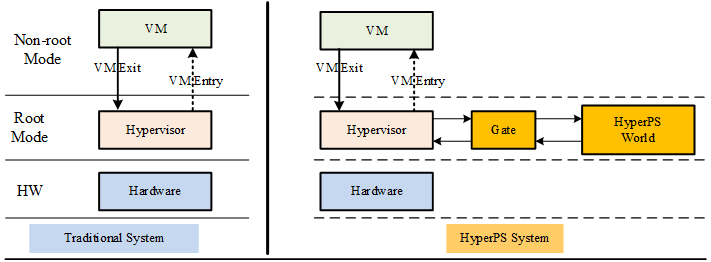
\includegraphics[height=1.80in]{figures/p5.png}}
	\caption{Interaction comparision.}
	\label{fg5_intr_compr}
\end{figure}

\textbf{EPT Monitoring.} Some functions, EPT creating, loading, walking and destroying, need access address of EPT. It can cause system suspend if they can not access the address of EPT. In order to ensure these functions can execute normally, HyperPS places hooks on these functions, then dispatches them to HyperPS World and handles appropriately. In the meantime, HyperPS avoids double mapping attack to ensure that there is only one virtual address mapping to one physical memory page during EPT updating, and handles remapping problems to ensure the content of page cleaned after page is swapped out. This will be described in detail later.

If EPT isolation among VMs can not be guaranteed, a malicious VM can load other VM’s EPT and access the memory data. It is important to ensure EPT isolation and one VM only access own corresponding EPT. To ensure one EPT for one VM, HyperPS creates the VM-Mark structure stored in HyperPS World as Table \ref{tb1_vmmark} described. It records VMID, EPTID, EPT Address and binds them together. VMID is created when the VM is created. EPTID and EPT Address is recorded as long as the EPT of current VM is created.

% Please add the following required packages to your document preamble:
% \usepackage{graphicx}
\begin{table}[htbp]
	\centering
	\caption{vm-Mark Table.}
	\label{tb1_vmmark}
	\resizebox{\textwidth}{!}{%
		\begin{tabular}{|c|c|c|l|}
			\hline
			\multicolumn{4}{|c|}{\textbf{VM-Mark Table}} \\ \hline
			\textit{Label} & VMID & EPTID & EPT\_Address \\ \hline
			\textit{Description} & The VM Identifier & The EPT Identifier & The Entry Address of EPT \\ \hline
		\end{tabular}%
	}
\end{table}

\textbf{VM Isolation.} Isolating memory is another aspect that should be considered. We need to ensure that the VM and the hypervisor can only access their own corresponding memory, as shown in Figure \ref{fg6_memiso}. Without memory isolation, a VM may suffer double mapping attack and remapping attack described in section \ref{subsec:thread_md}. We use Page-Mark structure described in Table \ref{tb2_pagemark} to record the owner and status of every page.

\begin{figure}[htbp]
	\centerline{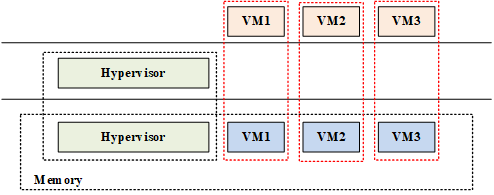
\includegraphics[height=1.20in]{figures/p6.png}}
	\caption{Memory isolation for VMs.}
	\label{fg6_memiso}
\end{figure}

% Please add the following required packages to your document preamble:
% \usepackage{graphicx}
\begin{table}[htbp]
	\centering
	\caption{Page-Mark Table}
	\label{tb2_pagemark}
	\begin{tabular}{|c|c|c|}
		\hline
		\multicolumn{3}{|c|}{\textbf{Page-Mark Table}} \\ \hline
		\textit{Label} & OwnerID & Used \\ \hline
		\textit{Description} & The Owner Identifier & Free or Used \\ \hline
	\end{tabular}
\end{table}

In order to go against the double mapping attack in the process of EPT updating, HyperPS should finish these two tasks: 1) It should verify the owner of pages when EPT updates. 2) It should mark the OwnerID field of Page-Mark structure for unused pages or thwart the mapping operation for used pages in case of malicious double mapping behavior. So page marking technique can divide all the pages into different catalogs: the pages of hypervisor or the pages of every VM.

To go against the remapping attack, HyperPS cleans the content of the page when the page is swapped out, so attackers can’t get the content of the page by the way of remapping. HyperPS clears the Page-Mark structure of the corresponding page.

\subsection{Security Guarantee for HyperPS World} \label{subsec:secugrant}
The security of HyperPS World guarantees the security of HyperPS, because it relies on HyperPS World to provide a trusted environment for VMCS and EPT monitoring. Nevertheless, without any protection measures, kernel page table in Normal World is not secure for four reasons: 1) Attackers can control page table with the highest privilege after hypervisor is compromised. 2) Attackers can bypass Switch Gate to break the security of HyperPS World. 3) Attackers with the highest privilege can free to execute privilege instructions to modify the value of privilege registers, such as CR0, CR3 and so on. 4) Attackers can carry out DMA attack to access address space of HyperPS World casually. We detail the protection measures to resist these four types of attacks below.

\textbf{Protecting Page Table.} There are three reasons for controlling the two sets of page tables: 1) To access casually or bypass HyperPS World, attackers can tamper normal page table to map address of HyperPS World or load malicious page table to CR3. 2) Attackers can cover the hooked functions, redirect the functions to malicious code and bypass HyperPS World. 3) To break HyperPS World, malicious kernel code in Normal World with execution permission can be executed to subvert HyperPS.

For the first attack, we remove all entries that map to HyperPS World from the page table in Normal World and deprive the ability to access CR3 of the kernel. For the second attack, we intercept the accessing operation to CR0 and maintain the WP bit as 1. We stick to W+X and maintain the code segment of hooked functions unwritable. For the third attack, we set the kernel code segment as NX (non-executable) when HyperPSWorld is running. For more security, we modify the kernel to configure these two sets of page table as read-only by setting the page tables page unwritable. This is necessary to prevent the page tables from being modified by attackers. Privilege instructions about page fault and setting pte are hooked and trapped to HyperPS World. Any write permission modification of two sets of page table must cause the kernel to page fault, then we dispatch page fault to HyperPS World to verify the correctness of address mapping.

\textbf{Worlds Switching Securely.} HyperPS creates Switch Gate between Normal World and HyperPS World by loading entry address of page table into CR3. In order to ensure switch security, we design the switch process as follows.

The switching process described in Figure \ref{fg4_addr_space} is as follows: 1) Save the kernel state to the stack including general registers and interrupt enable/disable status. 2) Clear the interrupt with the CLI instruction. 3) Load the page table to the register CR3. 4) Interrupt again. 5) Jump to the HyperPS World. For the exit process, the control flow returns to Normal World by performing the operations in the reverse order.

\textbf{Accessing Control Registers Securely.} The hypervisor without HyperPS is privileged and it can free to execute privilege instructions, so that it can write any value to the related control registers. 1) Malicious attackers can close DEP mechanism by modifying CR0, close SMEP mechanism by modifying CR4. 2) Kernel code can load a crafted page table to bypass HyperPS World by converting a meticulously constructed address of one page table to CR3. To prevent these, HyperPS deprives sensitive privilege instructions executed by the hypervisor, and dispatches captured events to HyperPS World. HyperPS World can choose how to handle this event, such as executing, issuing alerts or terminating the process.

\textbf{Resisting DMA Attack.} DMA operation is used by hardware devices to access physical address directly. Malicious attackers can read or write arbitrary memory regions including HyperPS World by DMA. Therefore, it is a crucial focus of intercepting direct access to physical pages belonging to HyperPS World by DMA operation. Fortunately, HyperPS employs IOMMU mechanism to avoid DMA attack, which can carry out access control for DMA access. Our approach adopts two policies: 1) We remove the corresponding mapping of the critical data from the page table which IOMMU uses. These critical unmapped data includes the entrance address of HyperPS, data recording VM-Mark structure used in EPT management and so on. 2) HyperPS intercepts the address mapping functions about I/O, verifies whether the address belongs to the address space of HyperPS World, then chooses to map or unmap.

Through the above security measures, HyperPS can be protected from being bypassed and being broken, thus providing a secure execution environment for hypervisor monitoring and VM protection.


\section{EVALUATION} \label{sec:evalu}
In this section, we first analyze the security guarantees provided by HyperPS. Then, we evaluate the performance overhead by running a set of benchmarks on both standard KVM and HyperPS.


\subsection{Security Analysis} \label{subsec:secuanal}
In this section, we elaborate the security evaluation on how HyperPS achieves hypervisor monitoring and memory isolation among VMs through monitoring VMCS and EPT manipulations. In addition, we analyze the security of HyperPS itself. Table \ref{tb3_pagemark_instance} shows the real attack instances in line with the above attack model.

\textbf{Modifying VMCS Attack.} We clarify the importance of protecting interaction data including VMCS in Section \ref{subsec:vmprotapp}. Firstly, VMCS is hidden in HyperPS World and cannot be accessed by hypervisor. Secondly, functions that can access VMCS are hooked into HyperPS World, therefore, no functions outside HyperPS World can access VMCS. Attackers cannot get location of VMCS and access it. This prevents attackers from tampering interaction data. We examine protection for VMCS by conducting several attack cases which are widely adopted in real world. The modifying VMCS attack, one of attack cases listed in Table \ref{tb3_pagemark_instance}, which tries to tamper the Guest CR3 field of VMCS, fails because it loses the access privilege to VMCS. According to the above analysis, attackers cannot conduct further attacks which rely on VMCS access.

% Please add the following required packages to your document preamble:
% \usepackage{graphicx}
\begin{table}[htbp]
	\centering
	\caption{Page-Mark Table.}
	\label{tb3_pagemark_instance}
	\resizebox{\textwidth}{!}{%
		\begin{tabular}{|l|l|}
			\hline
			\multicolumn{1}{|c|}{\textit{\textbf{Attack}}} & \multicolumn{1}{c|}{\textit{\textbf{Description}}} \\ \hline
			Modifying VMCS Attack & Load a crafted GUEST\_CR3 value \\ \hline
			CVE-2017-8106 & Load a crafted EPT value \\ \hline
			DMS Attack & Access HyperPS World by DMA \\ \hline
			Code Injection Attack & Inject code and cover hooked function to bypass HyperPS World \\ \hline
		\end{tabular}%
	}
\end{table}

\textbf{Subverting Memory Across VMs Attack.} The main attacks that attackers can execute on subverting memory are double mapping attack and remapping attack by modifying EPT entry. Firstly, double mapping attack succeeds by allocating memory pages that have already been owned by a hostile VM to a victim VM. Secondly, another challenge is page remapping attack by a compromised hypervisor from a victim VM to a conspiratorial VM. This attack involves remapping a private page to another virtual address. The absence of EPT in Normal World can prevent modification from attackers because they cannot access EPT in memory region directly.

We implement a real attack by exploiting CVE-2017-8106 in kernel version 3.12. A privileged KVM guest OS user accesses EPT, conducts attacks via a single-context INVEPT instruction with a NULL EPT Pointer. Attackers cannot implement successfully and incur EPT access fault because HyperPS hides the address of EPT in HyperPS World and hijacks the loading of EPT. HyperPS verifies the value of EPT to avoid loading NULL value. Therefore, HyperPS can avoid subverting memory across VMs including double mapping attack, remapping attack as well as malicious EPT access.

\textbf{Destroying HyperPS World.} HyperPS World is created by relying on new page table. We analyze the protection for HyperPS World from four aspects, page table modification attack, hooks redirection attack, register modification attack and DMA attack.
\begin{enumerate}
	\item Page Table Modification Attack: Page table protection has been introduced in section \ref{subsec:secugrant}. The entry address mapping of the HyperPS page table is deleted from the old page table to prevent the kernel from accessing HyperPS World directly through the page table mapping. When HyperPS World is active, the kernel code does not have any executable permissions to prevent attacking a process running in HyperPS world. Attackers may attack in two ways. First, attackers may try to directly access the new page table address on the kernel page table by virtual address mapping. When he accesses it, there is page fault due to the absence of virtual to physical address mapping. Second, attackers may run kernel code while HyperPS World is active to attack programs running in HyperPS World. This can be prevented because of the absence of executable privilege of kernel code.
	\item Hooks Redirection Attack: Due to the code of hooked functions including page table updating, control register access operations and VMCS operations, EPT operations, are writable-protection. Accessing CR0 register operation used to set W+X is controlled and page table updating used to change code execution privilege is limited, attackers cannot redirect hooked functions and bypass monitoring.
	\item Register Modification Attack: Some register access operations including CR0, CR3, CR4, are controlled and hooked to HyperPS World. HyperPS completes the update and monitoring of registers to ensure that the security mechanism is enabled while the system is running. Protection for page table, hooked functions and registers, plays a role mutually in protection for HyperPS.
	\item DMA Attack: DMA attack is described in detail in section \ref{subsec:secugrant}. Attackers can use this feature to read or corrupt arbitrary memory regions. DMA attack is not a threat to HyperPS, because HyperPS is inherently secure against DMA using IOMMU. We remove the corresponding mapping of the critical data from the page table which IOMMU uses. These critical unmapped data includes the entrance address of HyperPS, VMCS, EPT and VM-Mark structure. HyperPS intercepts the related functions of the DMA mapping and verifies that the physical address to be mapped is not within the scope of the critical data address during the DMA mapping process. DMA attack that aims at modifying the VM memory or the page tables can also be defeated.
\end{enumerate}


\subsection{Performance Evaluation} \label{subsec:perfeva}
In HyperPS, the hypervisor is modified so that HyperPS World is initialized during the boot up sequence. This includes creating a new memory page table for HyperPS, allocating memory pages. VM startup can cause memory allocation and I/O access. These processes introduce security accessing and verification for VMCS in HyperPS World during VM Exit/Entry sequence. The hypervisor is modified to place hooks upon some sensitive system resources, including control registers, page table, VMCS and EPT, introducing worlds switching overhead using Switch Gate.

In order to assess the effectiveness of all aspects of HyperPS, we conduct a set of experiments to evaluate the performance impact imposed by HyperPS against an original KVM system (the baseline). We run two groups of experiments, compare the performance overhead including regular benchmarks performance, Hyperbench benchmark benchmarks performance  and VM load performance. For simplicity, we only present the performance evaluation on a server with 64 cores and 32 GB memory, running at 2.0 GHz and guest VM with 2 virtual cores. The version of the hypervisor and guest VM is 3.10.1. Different experiments are based on different numbers of guest VMs with different memory size. This is described later in all kinds of tests. Both the original hypervisor and HyperPS systems have the same configuration except the protection supported by HyperPS. The deviation of these experiments is insignificant. All the experiments are replicated fifty times and the average results are reported here.

\textbf{Regular Benchmarks Performance.} In order to obtain the impact of HyperPS on the whole system, we measure HyperPS with microbenchmarks and application benchmarks. We use guest VMs with 1 GB memory size.

\begin{figure}[htb]
	\centerline{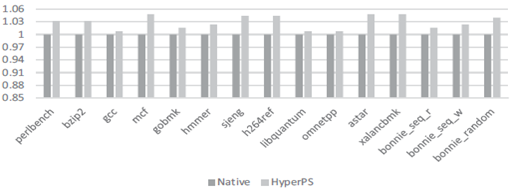
\includegraphics[height=1.70in]{figures/p7.png}}
	\caption{HyperPS Overhead Evaluation with Regular Benchmark.}
	\label{fg7_perfeva}
\end{figure}

To better understand the factor causing the performance overhead, we experiment with compute-bound benchmark (SPEC CPU2006 suite) and one I/O-bound benchmark (Bonnie++) running upon original KVM and HyperPS in Linux VMs. Figure \ref{fg7_perfeva} describes the results of SPEC CPU 2006 and Bonnie++ about the original KVM and HyperPS. The first 12 columns describe the results of SPEC CPU 2006 suite about Integer test and floating point test, and the last 3 columns describe the results of Bonnie++ about sequential read, write and random access. Most of the SPEC CPU2006 benchmarks (the first twelve groups) show less than 4.8\% performance overhead. It’s not surprising as there are few OS interactions and these tests are compute-bound. Mcf, astar, and xalancbmk with the highest performance loss allocate lots of memory. HyperPS verifies the legality of EPT when EPT updates. This can incur worlds switching which involves controlling register access and incur VM Exit which involves EPT updating. For Bonnie++, we choose a 1000 MB file to perform the sequential read, write and random access. The performance loss of sequential read, write and random access described in Figure \ref{fg7_perfeva} is 1.6\%, 2.4\% and 4\%, not high, the main reason is that HyperPS has no extra memory operations for I/O data. The performance result shows that HyperPS introduces trivial switch overhead of two worlds and trivial overhead of monitoring hypervisor.

\textbf{Hyperbench Benchmark Performance.} We use the Hyperbench that is a benchmark suite focuses on the capabilities of different virtualization platforms to measure HyperPS\cite{DBLP:journals/pomacs/WeiZT19}. The Hyperbench design 15 hypervisor benchmarks covering CPU, memory, and I/O. This benchmark test runs the script that the HyperPS load or unload 25 times on the Hyperbench test tool , each time 1 minute apart, the test results are as follows(Figure \ref{fg8_perftest_hb}):

\begin{figure}[htb]
	\centerline{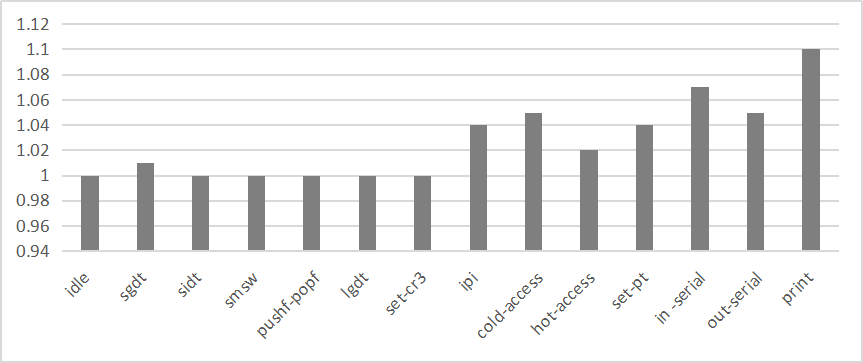
\includegraphics[height=1.70in]{figures/p8.png}}
	\caption{HyperPS Overhead Evaluation with Hyperbench.}
	\label{fg8_perftest_hb}
\end{figure}

The test is mainly to analyze whether the instructions of Hyperbench can cause VM exit and access to VMCS and EPT. As can be seen from the Figure \ref{fg8_perftest_hb}, the performance of the ipi, cold-access, set-pt, in-serial, out-serial, and print instructions has changed.

\begin{itemize}
	\item IPI. The virtual IPI involves many world switches between the VM and the hypervisor. First, the VM exit caused by writing ICR is necessary. Second, when the destination core receives this IPI, a VM exit will occur on a system that doesn’t have posted interrupts. When the posted-interrupt processing feature is enabled, the destination core receives the virtual IPI without a VM exit. So, this instruction can cause the VM exit.
	\item cold-access. When this instruction first accesses the data, the EPT update and VM exit can be triggered due to page missing.
	\item set-pt. This instruction is to set the page table mapping of the VM. After the mapping is set, when the VM accesses the GPA address, it can trigger EPT update and VM exit (access VMCS), so there will be some performance overhead when HyperPS runs.
	\item in-serial, out-serial, print. These instructions belong to IO access instructions, and can cause the VM to exit. So there can be some overhead.
\end{itemize}

In summary, HyperPS mainly changes VMCS and EPT and place the VMCS and EPT in another address space. This causes the data access time to be extended. The EPT update process and the validity of the verification map can result in an extended update cycle. But the overhead of testing these instructions is within reasonable limits.

\textbf{VM Loading Performance.} VM load time is a critical aspect of performance to be considered because it influences user experience. Experiments are done with 3 VMs, each guest VM is with different memory sizes from 512MB to 2GB. As expected, the VM booting time in HyperPS increases as the memory sizes increase, and the growth amplitude is larger due to the worlds switch and VMCS, EPT access. In addition, we measure the impact of completely booting and shutting down a VM (configured with 2 VCPU and 512MB memory). As Table \ref{tb4_exec_tm} shown, the booting time is suffered a 1.09 times slowdown under HyperPS, shutdown time is suffered a 1.07 times slowdown, due to the extra overhead of worlds switching and VM-Mark table accessing in HyperPS World.

\begin{table}[htbp]
	\centering
	\caption{Execution Time of VM Operation(s)}
	\label{tb4_exec_tm}
	\begin{tabular}{|l|c|c|}
		\hline
		\multicolumn{1}{|c|}{\textit{\textbf{Test Case}}} & \textit{\textbf{VM Create}} & \multicolumn{1}{l|}{\textit{\textbf{VM Destroy}}} \\ \hline
		No\_HyperPS & 10.54s & 2.34s \\ \hline
		With\_HyperPS & 11.49s & 2.50s \\ \hline
		Efficiency & 1.09 & 1.07 \\ \hline
	\end{tabular}
\end{table}

\section{RELATED WORK} \label{sec:relatwk}
We describe the related work from these three aspects, reconstructed hypervisor, customized hardware, and the same privilege-level isolation.

\subsection{Customized Hardware} \label{subsec:custmhdwr}
Some works at hardware level complete the protection of the process by extending the virtualization capabilities\cite{DBLP:conf/ccs/MoonLLKPK12},\cite{DBLP:journals/tdsc/LeeMHJJKPK19}. These tasks provide fine-grained isolation of processes and modules from the hardware level. Haven\cite{DBLP:journals/tocs/BaumannPH15} uses Intel SGX\cite{DBLP:conf/isca/HoekstraLPPC13},\cite{DBLP:conf/isca/McKeenABRSSS13} to isolate cloud services from other services and prevent cross-domain access. SGX provides fine-grained protection at the application space instead of hypervisor space, and needs developers spend time reconstructing code and dividing code into trusted part or untrusted part. SGX has requirement for version of CPU and is applied on a few platforms. Coplilot \cite{coplilot} use external hardware-based kernel integrity monitor based on memory snapshot inspection for static kernel regions. Vigilare\cite{vigilare}, Ki-Mon\cite{ki-mon} adopt the similar approaches to provide kernel integrity monitor.

\subsection{Reconstructed Hypervisor} \label{subsec:recnsthp}
Except for approaches based on hardware, some works \cite{DBLP:conf/ndss/ShiWXDCZL17},\cite{DBLP:conf/eurosys/SteinbergK10},\cite{DBLP:conf/eurosys/WangWGJ12} pay attention to software isolation. Pre-allocating physical resource and completed isolated environment for every VM can avoid VM cross-domain attack, and data leakage attack. NOVA \cite{DBLP:conf/eurosys/SteinbergK10} divides hypervisor into micro-hypervisor and user hypervisor running in root mode, adopts an idea which is similar to fault domain isolation to guarantee an isolated user hypervisor for every VM. The drawback of this approach is the lack of fractional traditional hypervisor functions. HyperLock \cite{DBLP:conf/eurosys/WangWGJ12} prepares backup KVM for every VM by copying KVM code, and ensures every VM run in own isolated space. These approaches redesign hypervisor greatly. In contrary, HyperPS adopts a feasible way to isolate VM without lots of modification of hypervisor.

\subsection{The Same Privilege Level Isolation} \label{subsec:tspli}
Some efforts, SKEE\cite{DBLP:conf/ndss/AzabSBMSWN16} and SecPod\cite{DBLP:conf/usenix/WangCWQZ15}, \cite{DBLP:conf/vee/DengLXCZ17}, adopt the same privilege-level idea to avoid performance overhead of inter-level translation. SKEE can only be applied to limited levels of system software in comparison with HyperPS. First, targeting ARM’s 32-bit architecture, SKEE capitalizes mainly on Translation Table Base Control Register (TTBCR) for dynamic page table activation. To be more specific, SKEE creates separate page tables for the secure world and activates it in a timely manner by modifying the N field of TTBCR. However, as this hardware feature is only defined in the kernel privilege level on AArch32, SKEE is not commonly applicable to different levels of system software, such as hypervisors. SecPod, an extensible approach for virtualization-based security systems that can provide both strong isolation and the compatibility with modern hardware. The biggest difference between SecPod and HyperPS is that SecPod creates the secure isolation environment for every VM. SecPod solves the problem of VM address mapping with the assistance of shadow page table (SPT) technology.

We neither adopt software at a higher level than the hypervisor, nor use customized hardware. Inspired by the same privilege-level, we propose HyperPS World placed at the same privilege-level with hypervisor. HyperPS is independent on multi-platforms and practical for cloud providers.


\section{CONCLUSION} \label{sec:conclsn}
We introduce HyperPS, a VM protection system to support hypervisor monitoring and VM memory isolation based on privilege separation. HyperPS World, the secure isolated execution environment, is designed to provide memory isolation protection for VMs, and event-driven runtime monitoring for interaction between hypervisor and VM. This approach, which does not rely on microhypervisor or a higher privilege level software, has fewer changes to system and fewer requirements for types of CPU hardware device. It reflects good practicality, portability, and independence on multi-platforms. We implement prototype system on x86 platform. And security analysis verifies the HyperPS achieves pre-defined security goals, the performance evaluation shows its efficiency by introducing negligible performance overhead. It can be implemented widely in real-world for cloud providers.

%\section*{References}

\bibliography{mybibfile}
\end{document}

